\section{Condenser Loop}\label{condenser-loop}

The condenser loop uses a cooling tower to supply cooling water to the water-cooled electric chiller in the chilled water loop. Hence, the supply side of this loop consists of the cooling tower and the demand side consists of the electric chiller. The schedules for this loop are almost identical to the ones applied on the CW loop. They dictate that the cooling tower also works around the year. The plant equipment schemes specify the cooling capacity/load of the cooling tower. The operation of the cooling tower is managed by monitoring the outdoor air wet bulb (air cooled condenser) temperature at the location of the simulation. The structure of this loop is very similar to that of the chilled water loop, the only difference being the main components in the loop. A simple line diagram of the condenser loop is provided in Figure~\ref{fig:simple-line-diagram-for-the-condenser-loop-002}.

\begin{figure}[hbtp] % fig 28
\centering
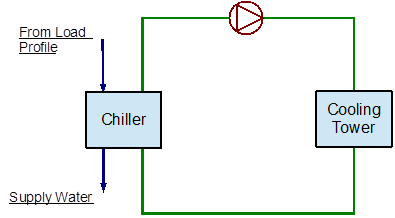
\includegraphics[width=0.9\textwidth, height=0.9\textheight, keepaspectratio=true]{media/image028.png}
\caption{Simple line diagram for the condenser loop \protect \label{fig:simple-line-diagram-for-the-condenser-loop-002}}
\end{figure}

\subsection{Flowcharts for the Condenser Loop Input Process}\label{flowcharts-for-the-condenser-loop-input-process-001}

As discussed in Section 1 the supply side and the demand side of the loop are modeled separately by following the process provided in the flow chart. The flow charts for this loop are provided below.

A \emph{PlantLoop} object is used to model the condenser loop with the chiller and the cooling tower as its main components. The working fluid is water. This loop is also sized such that the loop exit temperature is set to 20 degrees Celsius and the loop design temperature difference is 5 degrees Celsius. The chiller serves as the bridge between the chilled water loop and the condenser loop. This is achieved by managing the nodal connections on the chiller, hence the chiller appears on two branches in the system (supply branch of the CW loop, and the demand branch of the condenser loop). The EnergyPlus line diagram for the condenser loop is provided in Figure~\ref{fig:energyplus-line-diagram-for-the-condenser-002}. A simple flow chart for the separation of the half loops is provided in Figure~\ref{fig:simple-flowchart-for-separation-of-half-loops-001}.

\begin{figure}[hbtp] % fig 29
\centering
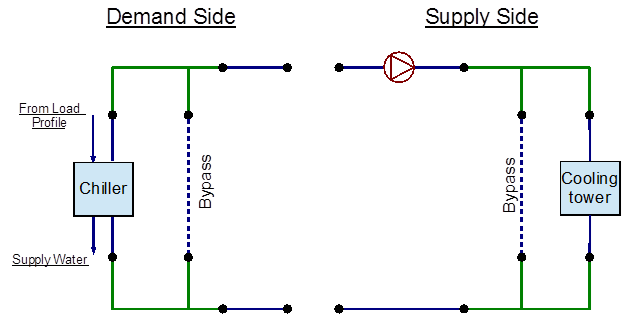
\includegraphics[width=0.9\textwidth, height=0.9\textheight, keepaspectratio=true]{media/image029.png}
\caption{EnergyPlus line diagram for the condenser loop \protect \label{fig:energyplus-line-diagram-for-the-condenser-002}}
\end{figure}

\begin{figure}[hbtp] % fig 30
\centering
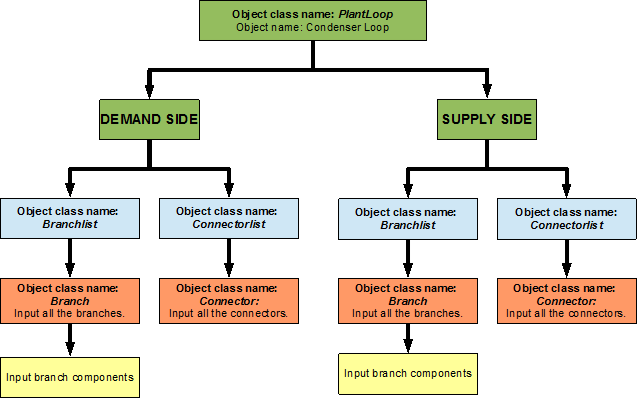
\includegraphics[width=0.9\textwidth, height=0.9\textheight, keepaspectratio=true]{media/image030.png}
\caption{Simple flowchart for separation of half loops in the condenser loop \protect \label{fig:simple-flowchart-for-separation-of-half-loops-001}}
\end{figure}

\subsubsection{Condenser Loop Supply Side Construction}\label{condenser-loop-supply-side-construction-001}

The main components in the supply side of the condenser loop are the condenser circulation pump and the cooling tower. The temperature set-point is set at the outlet node, where the outdoor air wet bulb temperature is monitored to regulate the operation of the cooling tower. The outdoor air conditions are obtained from the weather information file during the simulation. This side of the loop has eight nodes and four branches. An EnergyPlus diagram for the condenser loop supply side is provided in Figure~\ref{fig:energyplus-line-diagram-for-the-supply-side-003}. The flowchart for supply side branch definition is provided in Figure~\ref{fig:flowchart-for-condenser-supply-side-branches}. The flowchart for the supply side connectors is provided in Figure~\ref{fig:condenser-loop-supply-side-connectors}.

\begin{figure}[hbtp] % fig 31
\centering
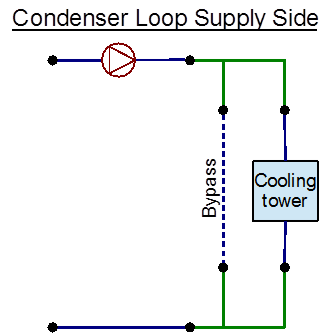
\includegraphics[width=0.9\textwidth, height=0.9\textheight, keepaspectratio=true]{media/image031.png}
\caption{EnergyPlus line diagram for the supply side of the condenser loop \protect \label{fig:energyplus-line-diagram-for-the-supply-side-003}}
\end{figure}

\begin{figure}[hbtp] % fig 32
\centering
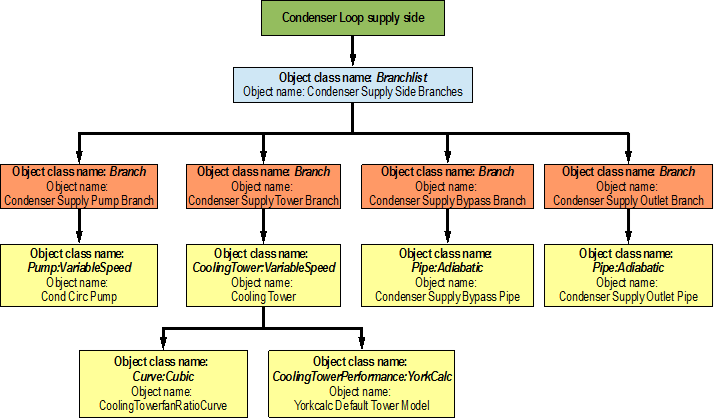
\includegraphics[width=0.9\textwidth, height=0.9\textheight, keepaspectratio=true]{media/image032.png}
\caption{Flowchart for condenser supply side branches and components \protect \label{fig:flowchart-for-condenser-supply-side-branches}}
\end{figure}

\begin{figure}[hbtp] % fig 33
\centering
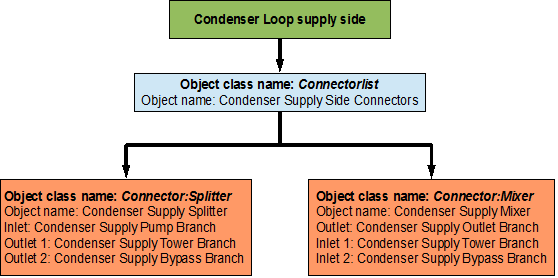
\includegraphics[width=0.9\textwidth, height=0.9\textheight, keepaspectratio=true]{media/image033.png}
\caption{Condenser loop supply side connectors \protect \label{fig:condenser-loop-supply-side-connectors}}
\end{figure}

\begin{center}\rule{0.5\linewidth}{\linethickness}\end{center}

\begin{center}\rule{0.5\linewidth}{\linethickness}\end{center}

\subsubsection{Condenser Loop Demand Side Construction}\label{condenser-loop-demand-side-construction-001}

The central component of the demand side is the chiller. The flowchart for the construction of the demand side is also provided below. The schedules for this side do not need to be specified, because the schedules that apply to the chiller also apply to this side of the condenser loop. This side of the loop also contains eight nodes and four branches. An EnergyPlus schematic for the demand side is provided in Figure~\ref{fig:energyplus-line-diagram-for-the-demand-side-2016-06-17}. The flowchart for demand side branch definition is provided in Figure~\ref{fig:condenser-loop-demand-side-construction}. The flowchart for the demand side connectors is provided in Figure~\ref{fig:condenser-loop-demand-side-schedules}.

\begin{figure}[hbtp] % fig 34
\centering
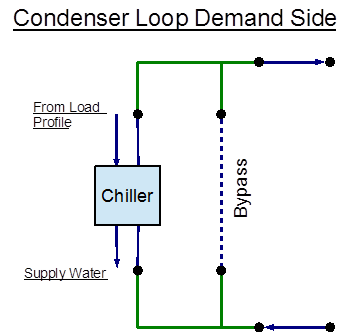
\includegraphics[width=0.9\textwidth, height=0.9\textheight, keepaspectratio=true]{media/image034.png}
\caption{EnergyPlus line diagram for the demand side of the condenser loop \protect \label{fig:energyplus-line-diagram-for-the-demand-side-2016-06-17}}
\end{figure}

\begin{figure}[hbtp] % fig 35
\centering
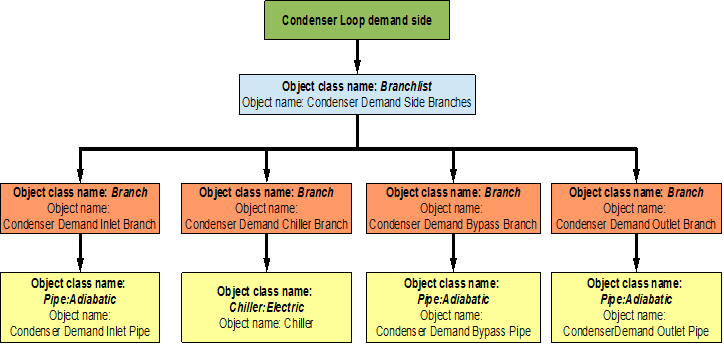
\includegraphics[width=0.9\textwidth, height=0.9\textheight, keepaspectratio=true]{media/image035.png}
\caption{Condenser loop demand side construction \protect \label{fig:condenser-loop-demand-side-construction}}
\end{figure}

\begin{figure}[hbtp] % fig 36
\centering
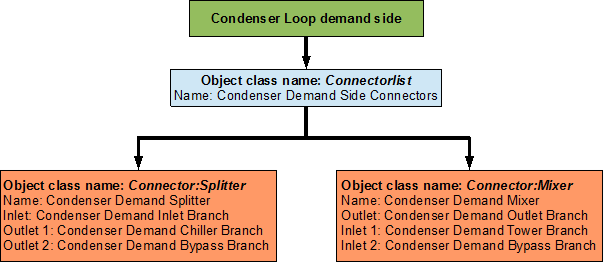
\includegraphics[width=0.9\textwidth, height=0.9\textheight, keepaspectratio=true]{media/image036.png}
\caption{Condenser loop demand side schedules, equipment schemes and setpoints \protect \label{fig:condenser-loop-demand-side-schedules}}
\end{figure}

\subsection{Flowcharts for Condenser Loop Controls}\label{flowcharts-for-condenser-loop-controls-001}

The cooling tower is also scheduled similar to the chiller because both of these units have to work together in order to satisfy the cooling load. The operation of the cooling tower is determined by using a set point at the condenser supply exit node. This set point monitors the temperature at this node as well as the outdoor air wet bulb temperature to operate the cooling tower. The flowchart for the schedules, plant equipment schemes, and the set points are also provided below.

\subsubsection{Condenser Loop Schedules}\label{condenser-loop-schedules-001}

The \emph{Tower AlwaysOnSchedule} is a compact schedule that keeps the tower ON at all times of the day for a whole year, this compact schedule uses a discrete \emph{scheduletypelimit} (\emph{Tower On/Off)} which defines that the value of On is 1 and that of Off is 0. A flowchart for condenser loop schedules is provided in Figure~\ref{fig:condenser-loop-schedules}.

\emph{~}

\begin{figure}[hbtp] % fig 37
\centering
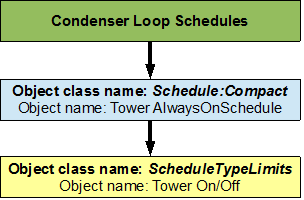
\includegraphics[width=0.9\textwidth, height=0.9\textheight, keepaspectratio=true]{media/image037.png}
\caption{Condenser loop schedules \protect \label{fig:condenser-loop-schedules}}
\end{figure}

\subsubsection{Condenser Loop Plant Equipment Operation Schemes}\label{condenser-loop-plant-equipment-operation-schemes-001}

The plant equipment operation schemes for the condenser loop are very similar to those of the chilled water loop. The \emph{PlantEquipmentOperationschemes} object uses the \emph{Tower AlwaysOnSchedule} and the \emph{Tower Load} objects to set the range of the demand loads for which the cooling tower is operated during the simulation period. A flowchart for the condenser loop plant equipment operation schemes is provided in Figure~\ref{fig:condenser-loop-plant-equipment-operation}.

\begin{figure}[hbtp] % fig 38
\centering
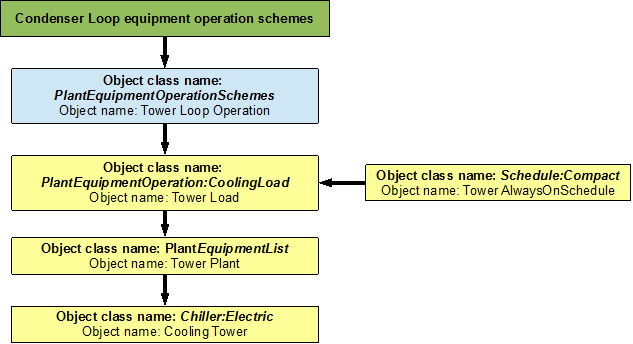
\includegraphics[width=0.9\textwidth, height=0.9\textheight, keepaspectratio=true]{media/image038.png}
\caption{Condenser loop plant equipment operation schemes \protect \label{fig:condenser-loop-plant-equipment-operation}}
\end{figure}

\subsubsection{Condenser Loop Setpoints}\label{condenser-loop-setpoints-001}

The \emph{Condensercontrol setpointmanager} places a temperature setpoint at the \emph{Condenser Supply Outlet Node.} The temperature at this point is controlled with respect to the outdoor air wet bulb temperature at that point in the simulation. The outdoor air wet bulb temperature is obtained from the weather data at the location of the simulation. A flowchart for the condenser loop setpoint is provided in Figure~\ref{fig:condenser-loop-setpoints}.

\begin{figure}[hbtp] % fig 39
\centering
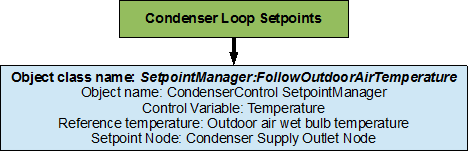
\includegraphics[width=0.9\textwidth, height=0.9\textheight, keepaspectratio=true]{media/image039.png}
\caption{Condenser loop setpoints \protect \label{fig:condenser-loop-setpoints}}
\end{figure}

\subsubsection{Condenser Loop Sizing}\label{condenser-loop-sizing-000}

The condenser loop is sized such that the loop exit temperature is 20 degrees Celsius and the loop temperature difference is 5 degrees Celsius. A flowchart for condenser loop sizing is provided in Figure~\ref{fig:condenser-loop-sizing}.

\begin{figure}[hbtp] % fig 40
\centering
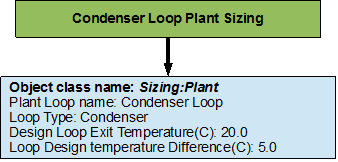
\includegraphics[width=0.9\textwidth, height=0.9\textheight, keepaspectratio=true]{media/image040.png}
\caption{Condenser loop sizing \protect \label{fig:condenser-loop-sizing}}
\end{figure}
